\PassOptionsToPackage{unicode=true}{hyperref} % options for packages loaded elsewhere
\PassOptionsToPackage{hyphens}{url}
%
\documentclass[
  12pt,
  a4paper,
  oneside]{book}
\usepackage{lmodern}
\usepackage{setspace}
\setstretch{1.5}
\usepackage{amssymb,amsmath}
\usepackage{ifxetex,ifluatex}
\ifnum 0\ifxetex 1\fi\ifluatex 1\fi=0 % if pdftex
  \usepackage[T1]{fontenc}
  \usepackage[utf8]{inputenc}
  \usepackage{textcomp} % provides euro and other symbols
\else % if luatex or xelatex
  \usepackage{unicode-math}
  \defaultfontfeatures{Scale=MatchLowercase}
  \defaultfontfeatures[\rmfamily]{Ligatures=TeX,Scale=1}
\fi
% use upquote if available, for straight quotes in verbatim environments
\IfFileExists{upquote.sty}{\usepackage{upquote}}{}
\IfFileExists{microtype.sty}{% use microtype if available
  \usepackage[]{microtype}
  \UseMicrotypeSet[protrusion]{basicmath} % disable protrusion for tt fonts
}{}
\makeatletter
\@ifundefined{KOMAClassName}{% if non-KOMA class
  \IfFileExists{parskip.sty}{%
    \usepackage{parskip}
  }{% else
    \setlength{\parindent}{0pt}
    \setlength{\parskip}{6pt plus 2pt minus 1pt}}
}{% if KOMA class
  \KOMAoptions{parskip=half}}
\makeatother
\usepackage{xcolor}
\IfFileExists{xurl.sty}{\usepackage{xurl}}{} % add URL line breaks if available
\IfFileExists{bookmark.sty}{\usepackage{bookmark}}{\usepackage{hyperref}}
\hypersetup{
  pdftitle={Spatial Machine Learning modelling: End-to-End web app solution},
  pdfauthor={Niccolò Salvini},
  pdfborder={0 0 0},
  breaklinks=true}
\urlstyle{same}  % don't use monospace font for urls
\usepackage[left=4cm, right=3cm, top=3cm, bottom=3cm]{geometry}
\usepackage{longtable,booktabs}
% Allow footnotes in longtable head/foot
\IfFileExists{footnotehyper.sty}{\usepackage{footnotehyper}}{\usepackage{footnote}}
\makesavenoteenv{longtable}
\usepackage{graphicx,grffile}
\makeatletter
\def\maxwidth{\ifdim\Gin@nat@width>\linewidth\linewidth\else\Gin@nat@width\fi}
\def\maxheight{\ifdim\Gin@nat@height>\textheight\textheight\else\Gin@nat@height\fi}
\makeatother
% Scale images if necessary, so that they will not overflow the page
% margins by default, and it is still possible to overwrite the defaults
% using explicit options in \includegraphics[width, height, ...]{}
\setkeys{Gin}{width=\maxwidth,height=\maxheight,keepaspectratio}
\setlength{\emergencystretch}{3em}  % prevent overfull lines
\providecommand{\tightlist}{%
  \setlength{\itemsep}{0pt}\setlength{\parskip}{0pt}}
\setcounter{secnumdepth}{5}
% Redefines (sub)paragraphs to behave more like sections
\ifx\paragraph\undefined\else
  \let\oldparagraph\paragraph
  \renewcommand{\paragraph}[1]{\oldparagraph{#1}\mbox{}}
\fi
\ifx\subparagraph\undefined\else
  \let\oldsubparagraph\subparagraph
  \renewcommand{\subparagraph}[1]{\oldsubparagraph{#1}\mbox{}}
\fi

% set default figure placement to htbp
\makeatletter
\def\fps@figure{htbp}
\makeatother

\usepackage{booktabs}
\usepackage{pdfpages}
\usepackage{amsthm}
\makeatletter
\def\thm@space@setup{%
  \thm@preskip=8pt plus 2pt minus 4pt
  \thm@postskip=\thm@preskip
}
\makeatother
\let\oldmaketitle\maketitle
\AtBeginDocument{\let\maketitle\relax}
\usepackage[]{natbib}
\bibliographystyle{apalike}

\title{Spatial Machine Learning modelling: End-to-End web app solution}
\author{\href{https://niccolosalvini.netlify.app/}{Niccolò Salvini}}
\date{14 settembre, 2020}

\begin{document}
\maketitle

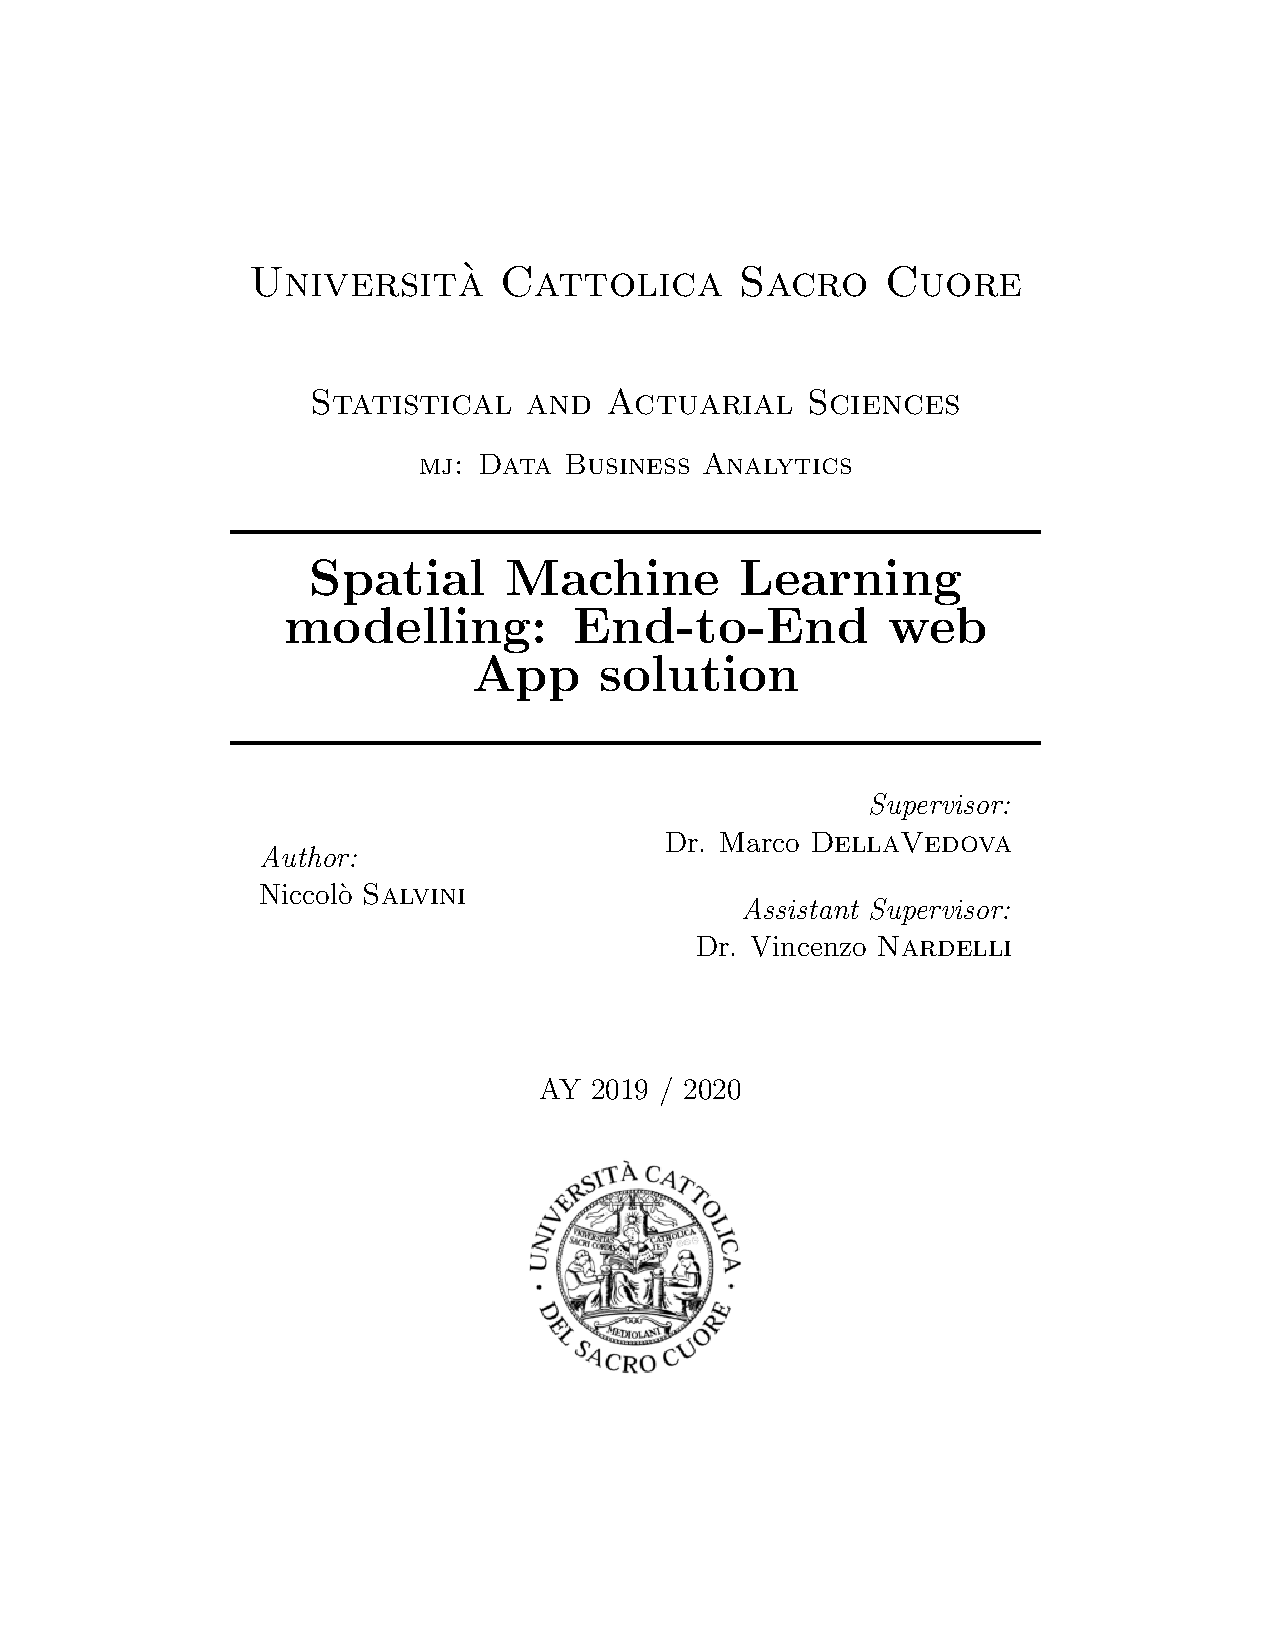
\includepdf[pages={1}, scale=1]{cover.pdf}
\newpage

\let\maketitle\oldmaketitle
\maketitle

{
\setcounter{tocdepth}{1}
\tableofcontents
}
\hypertarget{intro}{%
\chapter{Introduction}\label{intro}}

Main themes:

\begin{itemize}
\item
  (open data)
\item
  research question
\item
  milan market real estate
\item
  latest improvements in the subject matter
\item
  why both bayesian and non bayes methods
\item
\end{itemize}

We are living in the big data era, so we could be brought to think that evrething is a ``one click'' distant from us. Well, this is not totally true, moreover in some places this is truer. The main issue can be addressed to the lack of open data and the lack of relative infrastructure. This settings characterizes slow old economies and unfortunately Italy is one of them. Economies, and citizens on a later step, can largely benefit from public data and its usage. Some people in addition are in favour of the position that all data should be open.
Since I am living in italy and my \citep{lovelace_geocomputation_2019} goal is to an \citep{R-furrr} alyse market

The importance of data indeed justifies its accumulation and according to the latest reports is surpassing gold, despite these periods of uncertainity. The expression data is the new oil has neven been so appropirate in these times.
On the other hand is not for sure easy to assing a price amount to data due to its untangible nature.
the most straightfoprward and liberal approach could lead us to think that the price data should be exchanged the piceThe value attributed to data is not for sure self explanatory. It really depends on two major metrics: the usage that can be done through (with respect of the state of the art technology) it and the functionality with respect of other existing data. some data can be strategically important given the fact that someone already possess the complementary and can attribute some sort of competitive advantage. On the other hand as already been highlighted it really depends on the existing technology stack. Some data can be very useful but too costly either to process or to store.

During an interesting conversation with some friends we had a discussion on how data should be treated: as a sort of currency or a sort of commodity (raw material).
some people may say that the inner functioning is pretty much as a commodity. It gains value by its specialized usage and treatment. Sometimes a collection of data can represent the complementary part of a more general dataset that can not be used otherwise, in this analogy case a semifinished product. commodities sometimes are calmed, so that their prices are fixed to a certain amount, so it is for data, the

Durante una conversazione con alcuni amici

\begin{figure}

{\centering 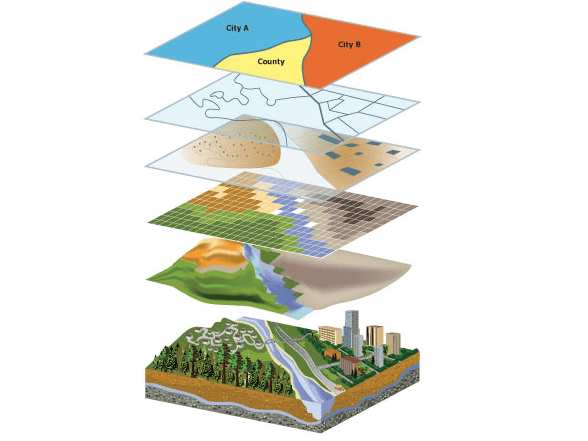
\includegraphics[width=8.17in]{images/spatial} 

}

\caption{API functioning}\label{fig:casuale}
\end{figure}

La ricerca che ho inteso fare sul mercato degli affitti a Milano mi ha aperto le porte a comprendere come poco digitalizzata e all'avanguardia sia la nostra amata penisola. L'indisposizione ai dati aperti, coperta da un sottile velo di ipocrisia chiamato privacy (ma quale?), ha reso non solo impossibile reperire i dati geospaziali tramite API di alcune aree dell'italia, ma ha reso necessario che costruissi delle funzioni che li estressero, appoggiandomi a cavilli. La questione è legale e relativaemnte complessa, e di certo la tesi non si indirizza a questi problemi, ma i dati che sono stato capace di scoprire e di farlo nella assoluta legalità si appoggiano ad una mancanza di autorizzazioni al trattamento che Immobiliare.it ha nel suo sito.
Un altro esempio di ritardo tecnologico riguarda l'assenza dei dati di elevazione su alcuni territori italiani.
Se per esempio immobilaire, come ha fatto un altro grosso player sul mercato, avesse apposto una checkbox obbigatoria da contrassegnare con relativi termini e trattamento dei dati io non avrei potuto accedere ai dati. La situazione aldifuori dell'italia è abbastanza uniforme, eccetto qualche paese noto come Germania e Francia, e meno noto come la Polonia, con tutte altre piattaforme e regole di trattamento dati. La domanda quindi sorge spontanea, perchè i dati degli italiani e degli europei sono meno accessibili dei dati degli americani?
Mentre in America è sufficiente richiamare un API con latitudine e longitudine della quadrettatura di terra necessaria per ottenere i dati di elevazione (.tif), in Italia l'unica soluzione è pagare google che tramite le sue private API è in grado di venderceli dietro autenticazione.
La risposta aldilà dei confini della legge presumibilmente risiede in un congiunturale ritardo di infrastrutture tecnologiche condivise e di indirizzo comune europeo sulla questione.
L'esigenza di dati aperti nasce per la risoluzione di problemi comuni a tutti, i dati sanitari hanno la missione di tentare risolvere problemi di natura sanitaria, i dati economici auspicabilmente curano probelmi o asimmentrie di un mercato. Il mercato degli affitti a Milano gode di sempiteerna gloria e ha visto la crescita degli affitti e dei prezzi degli immobili di paripasso al punto che una bolla è stata presunta. Diversi fattori hanno reso tale il fenomeno e diverse opinioni si sono spese sul tema. Alcuni pensano che dopo Expo la città abbia goduto di una spinta economia e innovativa che l'ha resa un'isola felice in mezzo ad un'italia che affanna. Altri ritengono che Milano goda di ottime infrastrutture, ma che la sua notorietà ed il suo appeal si sia sostituito a tutto quello che manca nelle altre città, ma che in Milano appare. La mia opinione è che sia una media di questi due pareri.
Un altro fattore è imporatante nella descrizione del fenomeno: l'asimmetria di infromazione tra chi cerca casa a Milano venendo da fuori e colui che affitta. Tale asimmetria viene ancora più esasperata al crescere della fretta che l'entrante ha nel trovare la locazione opportuna. La scelta diventa in molti casi antieconomica, nello specifico la domanda si genuflette all'offerta e accetta le svattaggiose condizioni proposte.
Infatti quello che appare certo è che i prezzi degli affitti se comparati ai salari per posizioni junior e di stage è falsato. Proprio qui nasce l'esigenza di approfondirne il perchè e fornire all'utente finale (un potenziale studente, un futuro lavoratore etc.) uno strumento che gli permetta di capire il prezzo stimato tramite predizione spaziale date le coordinate geografiche e gli attributi dell'appartamento e contestualmente fornire un mezzo di comparazione per altri immobili nelle vicinanze. Dall'altro lato dia un'idea chiara a chi vuole dare in affitto l'immobile, un prezzo rappresentativo, che ha fondamento nel modello utilizzato e nelle assunzioni che lo stesso modello impone alla realtà. Questo fa sì che da entrambi i lati ci sia trasparenza e che eventuali maggiorazioni di prezzo richiesto rispetto al sopradetto modello vengano penalizzate in favore di sconti applicati su altri immobili. Auspicabilmente i prezzi già gonfi si smusseranno in tutta la regione spaziale considerata, adattandosi alla domanda piuttosto che al capriccio dell'offerta.

\hypertarget{scraping}{%
\chapter{Scraping}\label{scraping}}

\citep{lovelace_geocomputation_2019, R-rvest}

Lo web scraping è una tecnica di estrazione dei dati da pagine internet statiche o dinamiche in maniera automatica e simulatanea \citep{wiki:xxx}. L'impossibilità di reperire dati aperti aggiornati riguardo l'affitto sul mercato italiano mi ha spinto a sviluppare sofisticate tecniche di estrazione di dati orientate ad alleggerire lo sforzo e aumentare la velocità di reperimento: da una parte nel preprocessing del dataset, nella successiva del fragente del modelling, per finire con la reattività di risposta dell'applicazione.
Le informazioni sui siti appaiono spesso ordinate e semplici, tuttavia ogni sito web ha una propria architettura e un proprio linguaggio. Per architettura intendo struttura gerarchica secondo cui è organizatto un sito internet: una semplificazione della struttura di un sito web può essere un insieme di cartelle innestate una dentro l'altra collegate tra loro da riferimenti tramite l'url. la natura gerarchica della struttura prevede che si usi un linguaggio che fa propria questa caratteristica, HTML è il preferito. L'html si organizza in nodi ed angoli, esattamente come un grafo; che aggiunta la componente gerarchica fa sì che questo sia un albero. Difatti spesso ci si riferisce alla struttura delle pagine web come html tree. Ogni elemento nella pagina ha un suo preciso posto nel codice sorgente della stessa e ha un preciso valore o più valori. Possiamo immaginare ogni nodo della pagina come una lista di valori che è collegata ad un nodo precedente detto padre da una struttura gerarchica superiore, ed eventiualmente ad un nodo successivo detto figlio. Pertanto tutte le informazioni che giacciono sotto al nodo padre sono parenti del nodo padre e sono direttamente collegate (directed nel senso dell'interpretazione), parallelamente ci saranno altri nodi padre che saranno adiacenti al nodo padre, i quali avranno nodi figli e così via.
La complessità della pagina e del codice è tanto maggiore quanto il livello dell'albero aumenta, tanto più l'albero è folto tanto più sarà difficile individurare il ramo o la foglia che ci interessa. Ragionevolemnte accade lo stesso per la funzione di scraping e il tempo di scraping.
Html organizza i contenuti e le relazioni tra loro, il css (Cascading Style Sheets) invece si occupa dello stile e della formattazione degli stessi. il css è uno strumento molto potente in mano ad uno scraper perchè permette di recuperare informazioni simili tra loro ma che occupano nodi con posizione gerarchica diversa all'interno della pagina. Pertanto una volta letto l'html della pagina sarà necessario recuperare la query css per raccogliere tutti gli elementi di interesse tramite la funzione di scraping.
Successivamente occorre notare che l'encoding da html a stringa di testo non è quasi mai lineare, spesso occorre riformattare, cancellare spazi, convertire la natura dell'oggetto estratto etc.
Il successivo elemento di complessità incontrato durante questa prima fase è stato interfacciarsi con un server attento alle richieste GET degli utenti. I dati viaggiano in pacchetti da un server che ospita un sito internet al nostro laptop. tutte le volte che cerchiamo di accedere ad un sito stiamo mandando una richiesta di ricezione di pacchetti dati ad un server in qualche luogo remoto del mondo. Quandi bussiamo alla porta del server se non siamo sospetti e superiamo i criteri autostabiliti dal server questo risponde, e lo fa con un numero che spazia da 200 a 500, due esempi: 200 se la risposta è positiva, 404 se la risposta è negativa. I criteri secondo cui gli utenti sono calssificati secondo utente normale o utente sospetto (aka bot) sono sintetizzati in un documento di testo chiamato robot.txt. Questo file di testo raccoglie tra le altre due infromazioni principali il delay time, cioè il tempo preferito dal server che deve intercorrere tra una richiesta dati e la successiva e quale utente è autorizzato ad accedere. Ogni utente posside un indirizzo IP che nelle richieste a server si codifica in user agent, cioè una stringa di testo dove vengono raccolte le infromzioni significative circa il dispositivo da cui provengono le richieste, un esempio:

`Mozilla/5.0 (Windows NT 10.0; WOW64) AppleWebKit/537.36 (KHTML, like Gecko) Chrome/54.0.2840.71 Safari/537.36',

dove ogni segmento della stringa rispecchia una caratteristica del laptop del richiedente, Chrome/54.0.2840.71 è la versione del browser chrome da cui proviene la richiesta Safari/537.36', è il motore di ricerca etc.

\begin{itemize}
\tightlist
\item
  Copia e incolla manuale
\item
  Web scraper
\item
  HTML parsing
\item
  Analisi con Visione computerizzata
\item
  DOM parsing
\item
  Riconoscimento dell'annotazione semantica
\item
  Aggregazione verticale
\item
  Text pattern matching
\end{itemize}

funzioni di scraping.

\hypertarget{Infrastructure}{%
\chapter{Infrastructure}\label{Infrastructure}}

The scraping functions, as they are designed, produce two .csv extension (if the boolean \texttt{write\ =\ TRUE}) files that should be joined by a primary key. But for the sake of
In order to gove the possibility to have a daily updated saptial analysis on data we need to continously have fresh data. In the website data come and go, as products in a marketplace, so the main idea is to have something that catches the new added and deletes what it is already taken.
Nowadays we have many open source, nearly cost free, techonlogies that allow us to have corporate grade applications that can be orizontally scaled at need. Most of them come with great docuemntation and ready to use examples that flatten the learning curve.
At frist a choice has to be made: either we provide a csv file day by day to feed the application, or we exploit some portable and fast solutions as API.

\textbf{(va prafrasato)}

API is a set of definitions and protocols for building and integrating application software. API stands for application programming interface.

APIs let your product or service communicate with other products and services without having to know how they're implemented. This can simplify app development, saving time and money. When you're designing new tools and products---or managing existing ones---APIs give flexibility; simplify design, administration, and use; and provide opportunities for innovation.

APIs are sometimes thought of as contracts, with documentation that represents an agreement between parties: If party 1 sends a remote request structured a particular way, this is how party 2's software will respond.

\begin{figure}
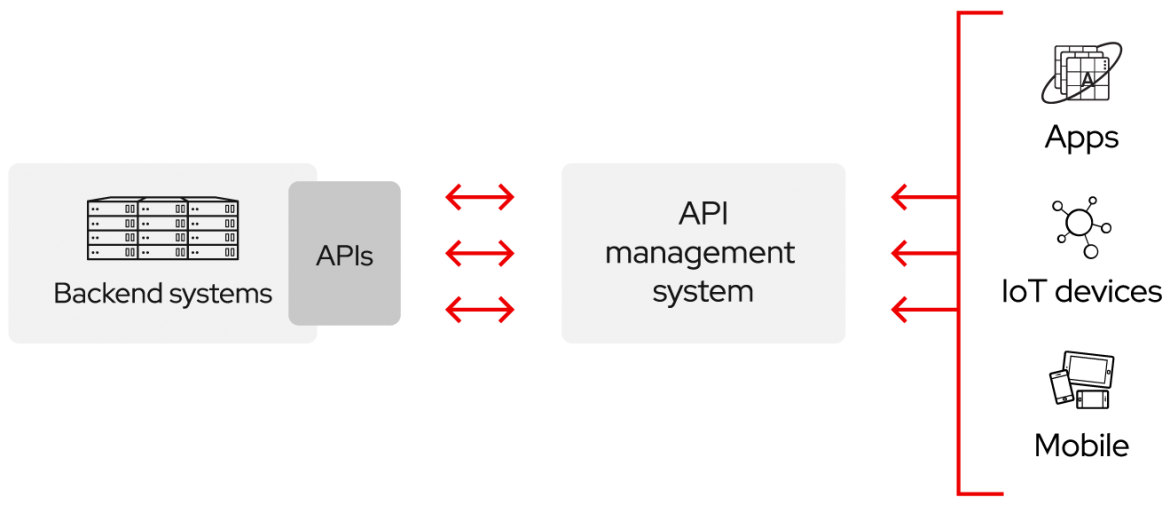
\includegraphics[width=16.25in]{images/API-page-graphic} \caption{API functioning}\label{fig:API}
\end{figure}

Because APIs simplify how developers integrate new application components into an existing architecture, they help business and IT teams collaborate. Business needs often change quickly in response to ever shifting digital markets, where new competitors can change a whole industry with a new app. In order to stay competitive, it's important to support the rapid development and deployment of innovative services. Cloud-native application development is an identifiable way to increase development speed, and it relies on connecting a microservices application architecture through APIs.

\begin{figure}
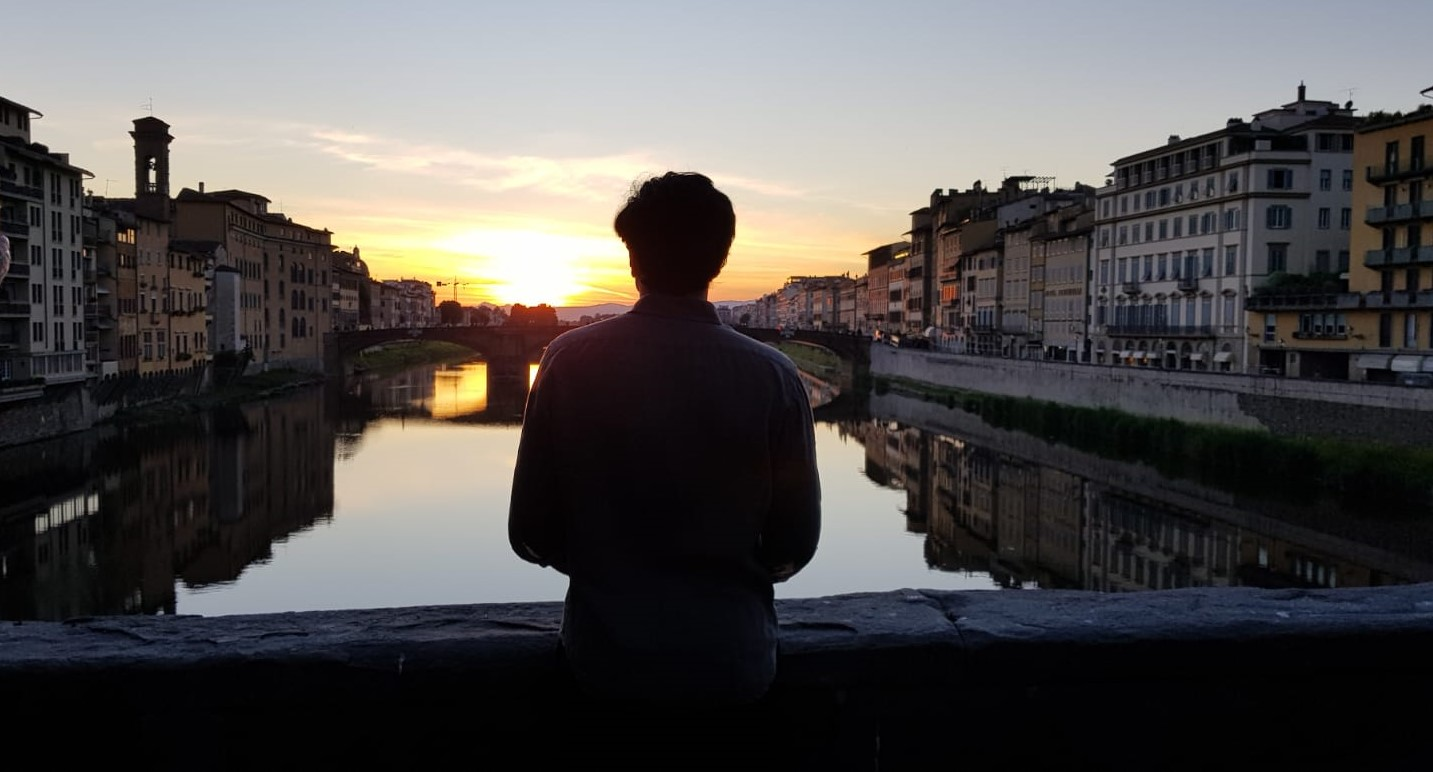
\includegraphics[width=19.9in]{images/FIRENZE} \caption{API functioning}\label{fig:nicco}
\end{figure}

\textbf{(va prafrasato)}

Since website are continously changed API philoposhy results in the best choice since it can be easily adapted to future changes

\hypertarget{methods}{%
\chapter{Methods}\label{methods}}

We describe our methods in this chapter.

Lorem ipsum dolor sit amet, consectetur adipiscing elit. Praesent sollicitudin arcu eget nulla convallis, in sagittis metus tincidunt. Integer vitae erat convallis, lobortis nunc id, commodo ipsum. Nam sem sem, tristique vitae dolor eget, laoreet aliquet libero. Nulla non feugiat diam. Ut vehicula, ante vitae rhoncus volutpat, eros orci viverra sem, ac tincidunt sem ex at sapien. Nam et odio condimentum, viverra nisl vitae, tempor nisl. Integer euismod convallis augue quis iaculis. Nulla at leo non nisi sollicitudin molestie vel at purus.

Nam tincidunt tellus et mattis luctus. Vivamus quis velit at nunc fermentum cursus. Duis elementum in nibh quis luctus. Suspendisse eget sem sit amet quam mattis egestas. Morbi ullamcorper metus eu dolor dapibus, id ultrices tellus euismod. Suspendisse malesuada felis vel tincidunt ullamcorper. Proin placerat auctor urna vel finibus. Sed non dictum orci. Ut volutpat pretium massa, in iaculis mi consectetur quis. Curabitur vitae condimentum nisi, sit amet consectetur justo. Curabitur non fermentum diam. Pellentesque vehicula laoreet elementum. Donec non porttitor ante, ut fermentum ante. In mollis consequat nisl euismod lobortis.

Vestibulum scelerisque dui eget est cursus, ut vestibulum libero pretium. Donec non viverra ligula. Suspendisse a viverra purus, in laoreet ligula. Nunc posuere libero ipsum, non vehicula massa gravida id. Interdum et malesuada fames ac ante ipsum primis in faucibus. Maecenas tortor risus, accumsan vitae luctus a, molestie non augue. Nam felis arcu, volutpat vitae eros nec, sollicitudin aliquam orci. Sed sit amet consectetur dui. Morbi finibus, est at blandit consectetur, diam massa ultrices libero, ac dapibus nisl ex id urna. Donec venenatis, nibh malesuada ultricies varius, justo tellus maximus ante, vehicula viverra dolor lorem vitae lacus. Donec nec ultricies ex. Proin vehicula interdum ex a tincidunt.

Duis varius ornare velit, non finibus purus lacinia eget. Fusce fringilla arcu in mauris fermentum, at consequat mauris suscipit. Etiam cursus felis ut consequat maximus. Vestibulum auctor sollicitudin nisl, eget molestie enim faucibus sit amet. Aenean luctus non ligula scelerisque maximus. Aenean finibus, nulla sit amet interdum ornare, justo nisl tempor diam, sit amet sollicitudin lacus tortor sit amet mi. Aliquam erat volutpat. Quisque vehicula facilisis ligula ut porta. Aenean eleifend arcu luctus ligula congue lacinia. Proin nunc mauris, cursus vel risus at, dapibus imperdiet est. Fusce eget nisi nec eros vehicula ullamcorper. Integer feugiat vulputate lacus id posuere. Nunc tincidunt, ante ac convallis elementum, ipsum elit rutrum risus, vitae dapibus augue leo in lacus.

Integer et aliquam mi, ac blandit arcu. Integer sit amet tristique orci. Aenean consectetur tempor diam, id finibus massa tempus non. Cras sagittis nibh vitae aliquet laoreet. Sed facilisis luctus mi. Donec est sapien, porta consectetur varius in, pulvinar sed ligula. Suspendisse potenti. Maecenas porta neque at accumsan eleifend. Proin porta imperdiet ipsum, sed viverra purus. Interdum et malesuada fames ac ante ipsum primis in faucibus. Mauris dapibus libero ac ultrices commodo. Donec dictum lectus id urna volutpat, vitae eleifend neque gravida. Mauris aliquam augue ac eros sagittis interdum. Sed dapibus placerat bibendum.

Lorem ipsum dolor sit amet, consectetur adipiscing elit. Sed imperdiet lacus ut maximus tempus. Integer dolor massa, ornare vitae ultrices pharetra, lacinia ut felis. Phasellus et vulputate mi, eu ultricies nisi. Phasellus interdum risus tristique tortor fermentum, blandit vehicula turpis elementum. Nullam eget arcu faucibus, blandit lacus ut, pharetra felis. Praesent malesuada mattis augue vel convallis. Curabitur sodales sollicitudin nunc, eget gravida risus condimentum non. Cras laoreet eget erat eget dapibus. Vivamus volutpat consequat libero at dapibus. Nulla convallis sapien neque, sit amet scelerisque enim luctus at. Praesent vehicula convallis purus. In a metus nec tellus mattis vestibulum. Vestibulum ultrices eleifend quam eu tincidunt.

Phasellus mauris elit, volutpat sit amet suscipit ut, scelerisque sed quam. Quisque maximus, justo non porta sollicitudin, ante lorem placerat nulla, nec commodo mi mauris eget risus. Interdum et malesuada fames ac ante ipsum primis in faucibus. Vestibulum ornare eleifend sem quis mollis. Proin vestibulum tristique erat, eu suscipit neque ornare et. Aenean scelerisque, nibh nec rutrum varius, justo nulla ultrices erat, non maximus mi massa vel mi. Integer ante arcu, accumsan vitae quam nec, faucibus cursus leo. Donec feugiat nunc quis orci ornare dignissim. Vivamus posuere enim et odio pretium, non tincidunt diam finibus. Praesent ut odio vitae magna euismod tempus. Ut laoreet nibh quis iaculis faucibus. Vivamus neque turpis, tempus ac orci id, volutpat laoreet nunc.

Nulla congue nunc elit, sit amet convallis urna lacinia eget. In massa erat, tempor eu erat ac, luctus sollicitudin felis. Curabitur urna ipsum, condimentum vel hendrerit a, imperdiet maximus ipsum. Morbi maximus malesuada efficitur. Phasellus id velit nec quam efficitur efficitur. Aenean a diam ut enim vehicula auctor ac nec sapien. Mauris in dapibus ex, quis consectetur ipsum. Lorem ipsum dolor sit amet, consectetur adipiscing elit. Curabitur at iaculis nulla. Aliquam turpis lacus, fermentum a malesuada eu, ornare sed libero. Fusce dictum fermentum ipsum, quis congue libero lacinia vel. Sed in finibus ligula. Vestibulum sagittis vel ex a mattis. Phasellus suscipit justo at augue porttitor pellentesque.

Nulla sed tellus vel nisl rutrum mattis a et est. Aenean dolor nunc, placerat quis enim a, fermentum malesuada enim. Aliquam erat volutpat. In ut est non velit vehicula hendrerit. Pellentesque eu erat finibus, viverra velit ac, tempus odio. Suspendisse potenti. Curabitur vulputate metus non ligula maximus sollicitudin. Donec facilisis augue sed urna lobortis, eu tempus mi ultrices. Aliquam fringilla sagittis felis, ac commodo arcu porttitor at. Ut lorem ex, gravida a porttitor in, feugiat vel ex. Aliquam consequat finibus ante, sed commodo sem. Ut ac mollis dui. Curabitur nec eros congue, pulvinar quam at, tincidunt dolor. Lorem ipsum dolor sit amet, consectetur adipiscing elit. Phasellus eu elit vulputate, scelerisque felis ut, accumsan nunc.

In non odio et risus rhoncus viverra nec in odio. Ut viverra metus eget nisi molestie sodales. Vestibulum ligula felis, malesuada quis vehicula eu, bibendum finibus diam. Donec ut rhoncus odio, tristique sodales orci. Praesent a ex lectus. Maecenas tristique sapien lorem, vel lobortis lorem porta sodales. Suspendisse ligula justo, iaculis id lorem eu, consequat vulputate lectus. Nunc molestie lacus at elit tempor, at rhoncus justo hendrerit. Nullam luctus lectus ac orci interdum, vitae varius libero pellentesque. Nunc lacinia erat lectus. Sed sit amet venenatis quam. Mauris interdum mauris sem, sit amet interdum eros tincidunt a.

Nam at dolor dui. Praes ent efficitur leo erat, id blandit neque ultrices non. Morbi eget dignissim eros. Praesent rhoncus maximus accumsan. Quisque et consectetur odio, id vehicula leo. Integer tempor diam augue, nec rhoncus ex suscipit id. Sed nec tempor tellus. Lorem ipsum dolor sit amet, consectetur adipiscing elit. Morbi feugiat tincidunt tortor quis efficitur. Maecenas pellentesque dapibus nisi, sed commodo augue. Fusce condimentum dignissim quam id feugiat. Mauris maximus ex vel enim viverra, eget placerat massa consectetur. Integer pellentesque finibus ipsum, quis vestibulum elit ultrices a. Vivamus nunc velit, lobortis at hendrerit non, laoreet nec urna.

Vestibulum ullamcorper, lacus sed malesuada porta, lectus nisi lacinia augue, at mollis lorem purus sit amet metus. Quisque et mauris leo. Donec id risus id nisl auctor gravida. Suspendisse sed tempor risus. Integer ornare sem quis turpis accumsan finibus. Morbi in ex dui. Lorem ipsum dolor sit amet, consectetur adipiscing elit. Nam id laoreet erat. Curabitur tempor faucibus turpis, a bibendum turpis dignissim tempor.

\hypertarget{applications}{%
\chapter{Applications}\label{applications}}

Some \emph{significant} applications are demonstrated in this chapter.

\hypertarget{example-one}{%
\section{Example one}\label{example-one}}

\hypertarget{example-two}{%
\section{Example two}\label{example-two}}

\hypertarget{final-words}{%
\chapter{Final Words}\label{final-words}}

We have finished a nice book.

  \bibliography{book.bib,packages.bib}

\end{document}
